\chapter{Begriffe}
    

%\printglossaries 

\begin{table}[htbp]
\begin{tabular}{ll}
Problem & \\
Störung & \\
Fehler & \\
Modul & \\
PFE & \\
Ziele & \\
\end{tabular}
\end{table}

\chapter{Anhang Analyse}

\todo{Zustandsdiagramm Services}

\chapter{Anhang Konzept}
\section{Farbschema}

\section{Anpassung an Problembereich - Aktivitätsdiagramm}
\todo{Aktivitätsdiagramm erstellen}

\begin{figure}[htbp]
\centering
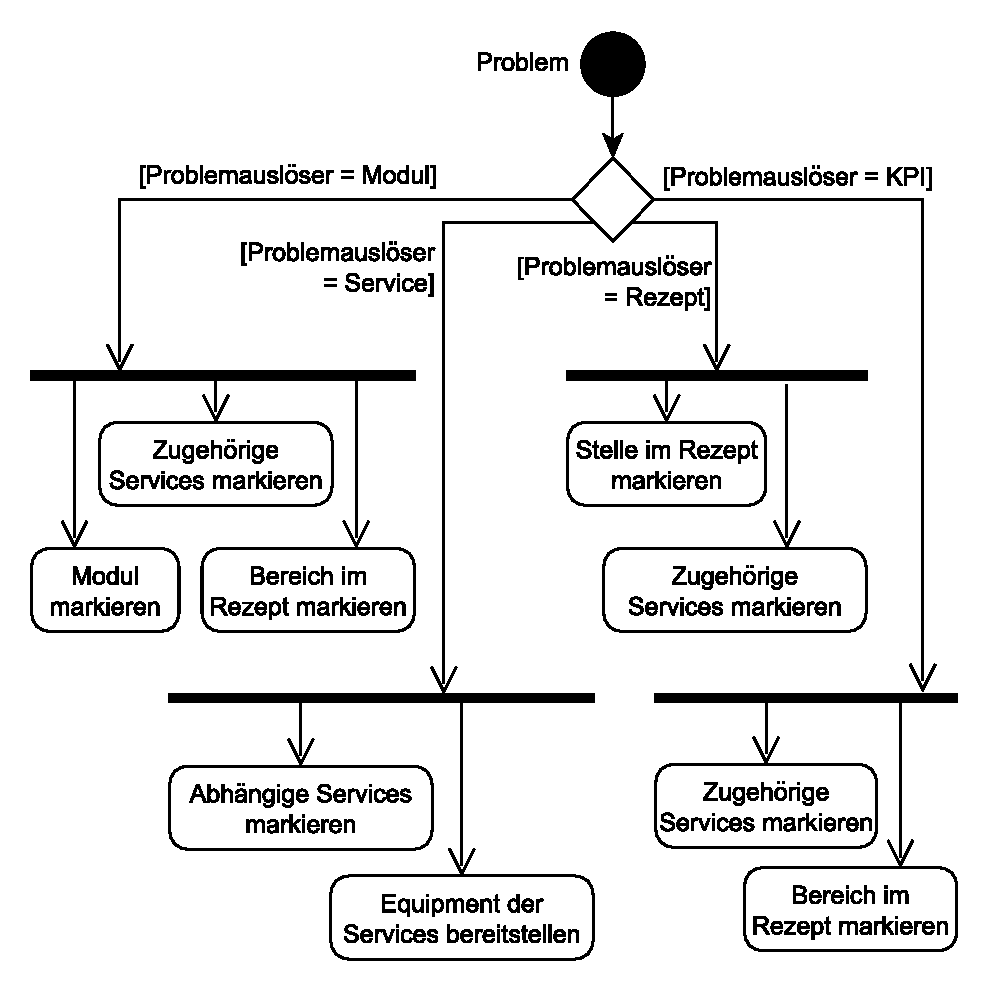
\includegraphics[angle=90,scale=0.6]{DA_files/UML/Anhang/Aktivitaetsdiagramm-Problem.pdf}
\caption{Aktivitätsdiagramm Anpassung an Problemauslöser}
\end{figure}

\chapter{Anhang Validierung}
\section{Fragebogen User Experience}

\begin{table}[htbp]
\caption{Fragen zum Vorwissen}
\centering
\begin{tabular}{|p{0.6 \textwidth}|l|l|}
\hline
Frage & Ja & Nein \\
\hline
Wissen Sie, was eine modulare Anlage ist? & & \\
\hline
Wissen Sie, was Services im Kontext der modularen Anlage sind? & & \\
\hline
Haben Sie Erfahrungen im Betrieb von verfahrenstechnischen Anlagen? & & \\
\hline
Wissen Sie, wie Rezepte bei verfahrenstechnischen Anlagen funktionieren? & & \\
\hline
Haben Sie schon mal Assistenzsysteme zum Problemlösen verwendet? & & \\
\hline 
\end{tabular}
\end{table}

%\subsection*{SUS-Fragebogen}
\begin{table}[htbp]
\caption{SUS-Fragebogen}
\centering
\begin{tabular}{|p{0.4 \textwidth}|p{0.15 \textwidth}|p{0.04 \textwidth}|p{0.04 \textwidth}|p{0.04 \textwidth}|p{0.1 \textwidth}|}
\hline
\textbf{Aussage} & Stimme gar nicht zu & & & & Stimme voll zu \\
\hline
Ich kann mir sehr gut vorstellen das Assistenzsystem regelmäßig zu nutzen. & & & & & \\
\hline
Ich empfinde das Assistenzsystem unnötig komplex. & & & & & \\
\hline
Ich empfinde das Assistenzsystem als einfach zu nutzen & & & & & \\
\hline
Ich denke, dass ich technischen Support brauchen würde, um das Assistenzsystem zu nutzen. & & & & & \\
\hline
Ich finde, dass die verschiedenen Funktionen des Assistenzsystems gut integriert sind. & & & & & \\
\hline
Ich finde, dass es im Assistenzsystem zu viele Inkonsistenzen gibt. & & & & & \\
\hline
Ich kann mir vorstellen, dass die meisten Leute das System schnell zu beherrschen lernen. & & & & & \\
\hline
Ich empfinde die Bedienung als sehr umständlich. & & & & & \\
\hline
Ich habe mich bei der Nutzung des Assistenzsystems sehr sicher gefühlt. & & & & & \\
\hline
Ich musste eine Menge Dinge lernen, bevor ich mit dem Assistenzsystem arbeiten konnte. & & & & & \\
\hline
\end{tabular}
\end{table}

Offene Fragen \todo{Offene Fragen}